\subsubsection*{Picture table}
Tabellen indeholder billeder og informationer om de billeder taget af dronen. Billeder gemmes i en blob type, som er binær-data i databasen.
\vspace{-5pt}
\begin{figure}[H]
	\centering
	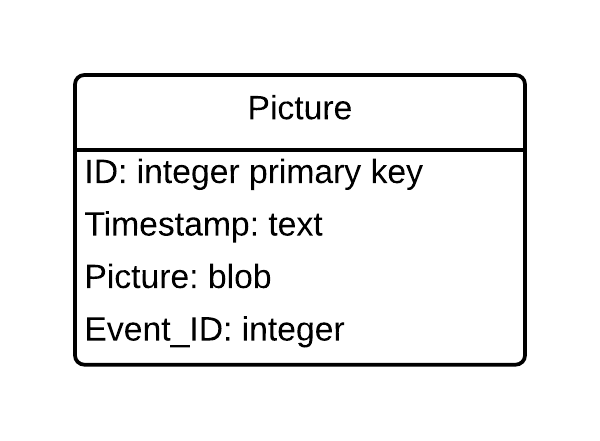
\includegraphics[width=0.5\textwidth]{Billeder/database/PictureTable.png}
	\vspace{-5pt}
	\caption{Picture table}
	\label{fig:picture_table}
\end{figure}

\begin{table}[H]
\begin{tabular}{| p{3cm}| p{11.5cm}|}
\hline

Formål	 							& Holde data om billeder i systemet og selve billederne.\\\hline
Forbindelser						& Picture tabellen har en foreing key til event tabellen.\\\hline
Attributter						& \begin{itemize}
												\item ID: Primary key.
												\item Name: Navnet på det givet event. Max length: 100 char
												\item Timestamp: Timestamp for oprettelse: Datefield
												\item Picture: blob: Udefinerbar størrelse binær data
												\item Event ID: Relation til event tabellen: Foreing key
											\end{itemize} \\\hline 
\end{tabular}
\caption{Picture table}
\label{tab:picture_table}
\end{table}